\begin{document}



The CD4007UBE integrated circuit will be modeled using NGSpice in conjunction with MATLAB for this purposes of the simulations for the signal generator. In Figure \ref{fig:cd4007_inside}, the pin connections for the IC as well as the internal design of the NMOS and PMOS MOSFETS connections. 

\begin{figure}[H]
    \centering
        \centering
        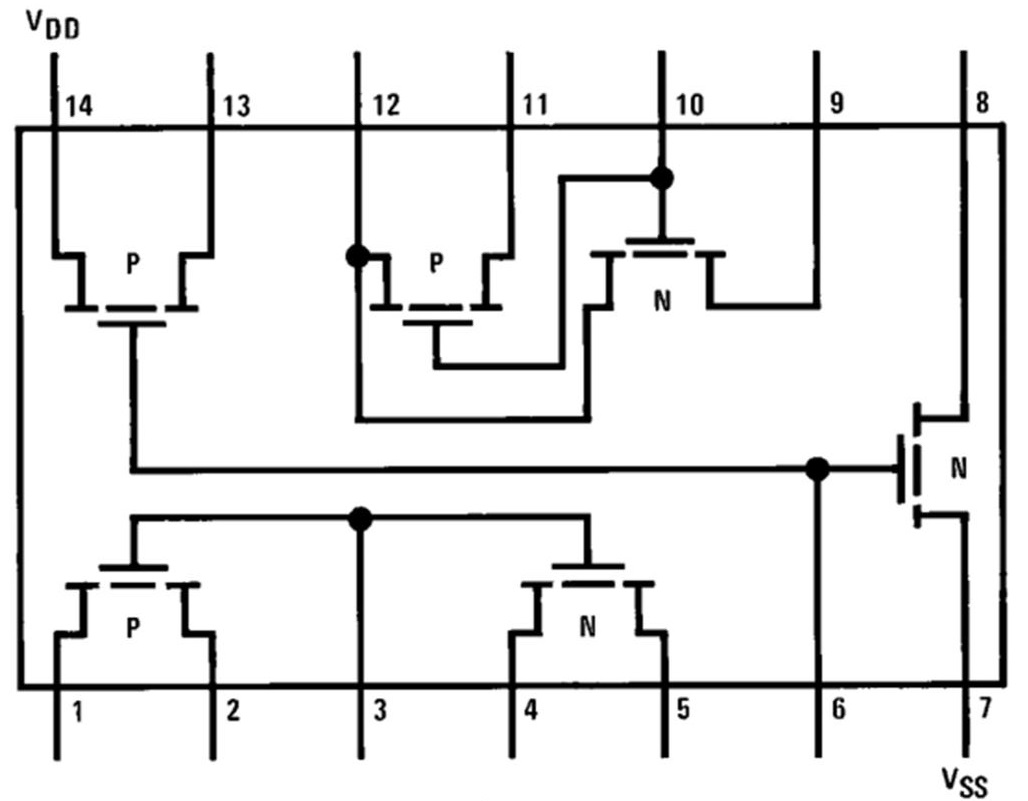
\includegraphics[scale = .7]{CircuitDevelopment/cd4007SIM/cd4007_Inside.jpg}
        \caption{CD4007UBE internal schematic}
        \label{fig:cd4007_inside}
\end{figure} 




\noindent There are two circuits that will be simulated. The first simulation is a CMOS inverter. The second simulated circuit will be a CMOS ring oscillator. Each of these simulations will be based on the design of the CD4007UBE IC. The CD4007UBE has three NMOS and PMOS transistors connected in pairs. The first two pairs have their gates connected to each other while the third pair have their gates and drains connected together. The third pair is best for implementing a single inverter due to it's connections.  


\subsubsection{CMOS inverter}

\noindent The design of the CMOS inverter will consist of a pair of MOSFETS, one being a PMOS and one being an NMOS connected in series between $V_{DD}$ and the reference, $GND$. The simulation schematic is shown in Figure \ref{fig:cmosinvert} below.
\begin{figure}[H]
    \centering
        \centering
        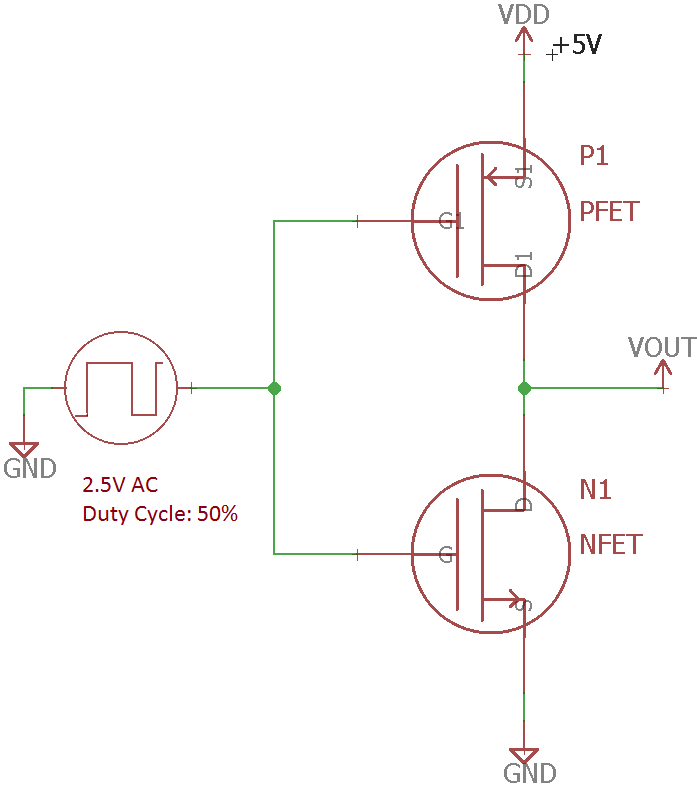
\includegraphics[scale = .35]{CircuitDevelopment/cd4007SIM/CMOSInevrter.png}
        \caption{CMOS inverter schematic}
        \label{fig:cmosinvert}
\end{figure} 

Based on the characteristics of the CMOS inverter circuit, which contains a PMOS and NMOS, a load-line plot can be drawn representing the voltage transfer function characteristics, VTC. This graphical interpretation is shown below in Figure \ref{fig:VTCchar}.

\begin{figure}[H]
    \centering
        \centering
        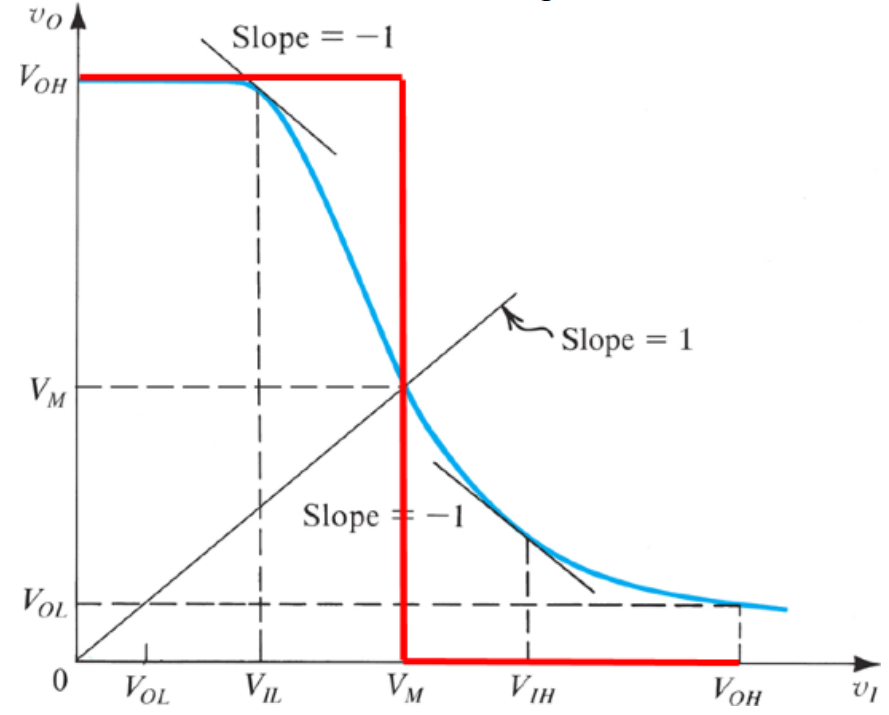
\includegraphics[scale = .25]{CircuitDevelopment/cd4007SIM/VTCInverter.png}
        \caption{Voltage transfer function characteristics}
        \label{fig:VTCchar}
\end{figure} 

In the first region of the VTC inverter graph, between 0 and before $V_{IL}$, known as the input voltage at the low logic state, the PMOS device is on. This is due to a low voltage being applied to it. The NMOS is essentially a large resistor  because it has no use of free electrons, which disallows conduction. As a result, there is no current flowing through the inverter, so the output voltage is equivalent to supply voltage, $V_{DD}$, because there is no voltage drop across the PMOS. Once the voltage reaches $V_{IL}$, the NMOS is already on and saturated because of a large $V_{DS}$ value. \newline

At $V_{IL}$, the slope of the VTC is $-1$, which is the maximum input voltage in this state. Afterwards, there is a point in the VTC at $V_M$ where $V_I = V_O$. This is the gate threshold voltage. At this time, the voltage dropped across the PMOS and NMOS are the same, and are both in a saturated state. In the area after the point $V_M$, the NMOS is conducting linearly, and the PMOS is being driven to saturation. The minimum voltage input at the high logic state occurs at $V_{IH}$, where the slope of VTC is once again $-1$ . 

After $V_{IH}$, the NMOS will still technically be conducting, but the drain current is too small due to a small leakage current from the PMOS. In real world applications, this value is extremely small and negligible. In the case of CMOS inverters, $V_{OH} = V_{DD}$ at this stage. The simulated VTC matches the expected VTC graph as shown below in Figure \ref{fig:VTCsim}.

\begin{figure}[H]
    \centering
        \centering
        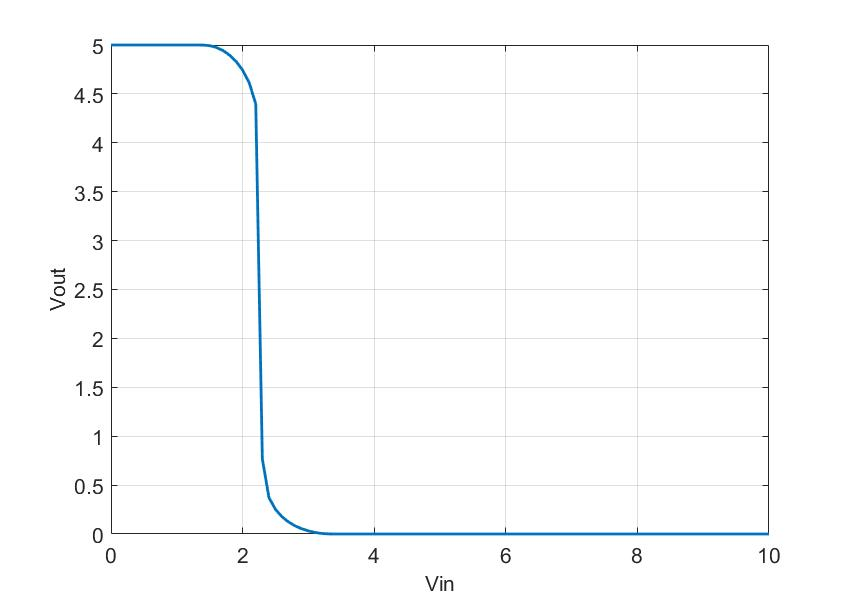
\includegraphics[scale = .25]{CircuitDevelopment/cd4007SIM/cmos_vtc.jpg}
        \caption{Voltage transfer characteristics - simulated}
        \label{fig:VTCsim}
\end{figure} 

The simulated VTC graph shows voltage input at the low logic state, $V_{IL}\approx 0V$ and the input at high logic state, $V_{OH}\approx 5V$. The voltage output is essentially the same as the voltage input to the gate except it is inverted. This means that when the input is high, the output will be low and when the input is low, the output will be high. However, the input pulse wave has virtually no rise and fall time for the purposes of this simulation. The output, due to constraints places on it by the characteristics of MOSFETS, will have a rise and fall time for each pulsed wave. These can be seen in Figure \ref{fig:VoutInvert}. 

\begin{figure}[H]
    \centering
        \centering
        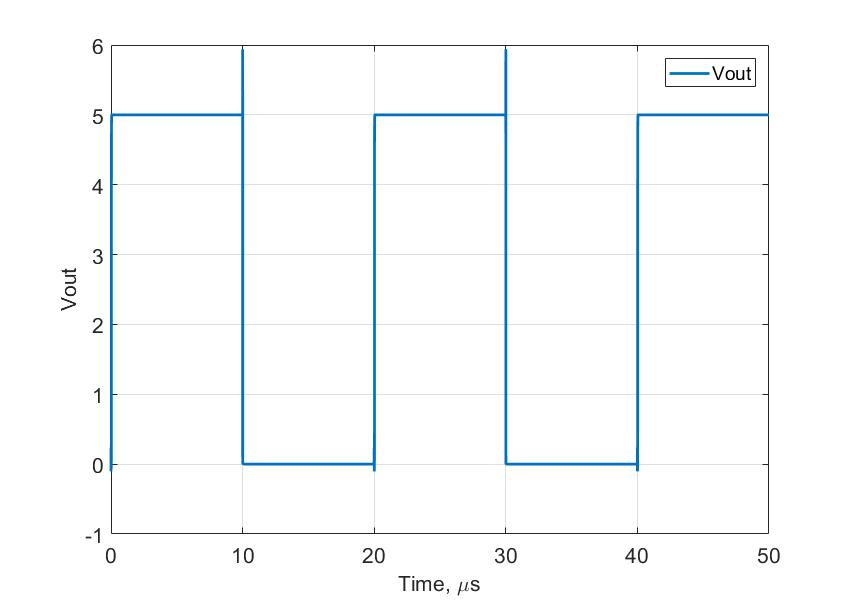
\includegraphics[scale = .3]{CircuitDevelopment/cd4007SIM/Vout_cascade_cmos.jpg}
        \caption{CMOS inverter voltage output}
        \label{fig:VoutInvert}
\end{figure} 

From the graph, the rise time is calculated as 142ns, while the fall time is calculated at 114ns. 

\subsubsection{CMOS astable multivibrator}

The astable multivibrator is another circuit providing an oscillating output. The unique quality that this circuit has, compared to others, is that it has no stable state. Instead, it is in a continuously switching state. This is due to the feedback network which returns the output voltage to the gate of the first inverter, which in turn, causes the state of the input to switch. The oscillation frequency can be altered by the charge and discharge rates of the RC circuit. The operating frequency for the astable multivibrator is described by Equation \ref{eqn:astablefreq} \cite{b3} 

\begin{equation}
f = \frac{1.44}{RC},
\label{eqn:astablefreq}
\end{equation}

where the frequency is inversely proportional to resistance and capacitance. The constant 1.44 is a coefficient resulting from the derivation of Equation \ref{eqn:astablefreq} \cite{b3}.  The resistance can then be solved for in Equation \ref{eqn:astablefreq}, with an additional factor of three being added, due to three stages, to result in Equation \ref{eqn:Rastable}.

\begin{equation}
R = \frac{1.44}{3fC},
\label{eqn:Rastable}
\end{equation}
R is found to be 24k$\Omega$ when C is set to 1nF. The schematic for the astable multivibrator using a CMOS is shown in Figure \ref{fig:cmosaschtable}.

\begin{figure}[H]
    \centering
        \centering
        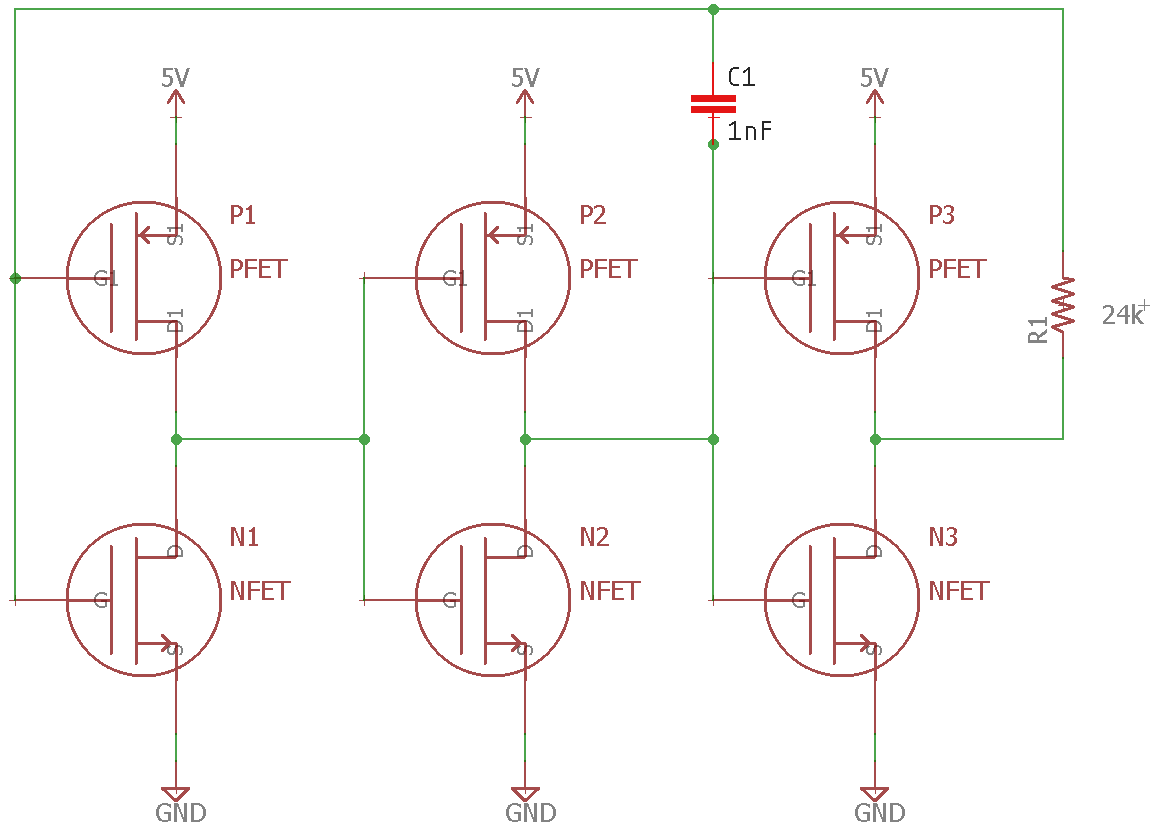
\includegraphics[scale = .35]{CircuitDevelopment/cd4007SIM/Aschtable.png}
        \caption{CMOS astable multivibrator schematic - simulated}
        \label{fig:cmosaschtable}
\end{figure} 
The resulting waveform is found by using transient analysis in NGSpice, which is shown in Figure \ref{fig:astablesingle}. The frequency was found to be approximately 19kHz. Subsequently, sensitivity testing was performed on the astable multivibrator using NGSpice.

\begin{figure}[H]
    \centering
        \centering
        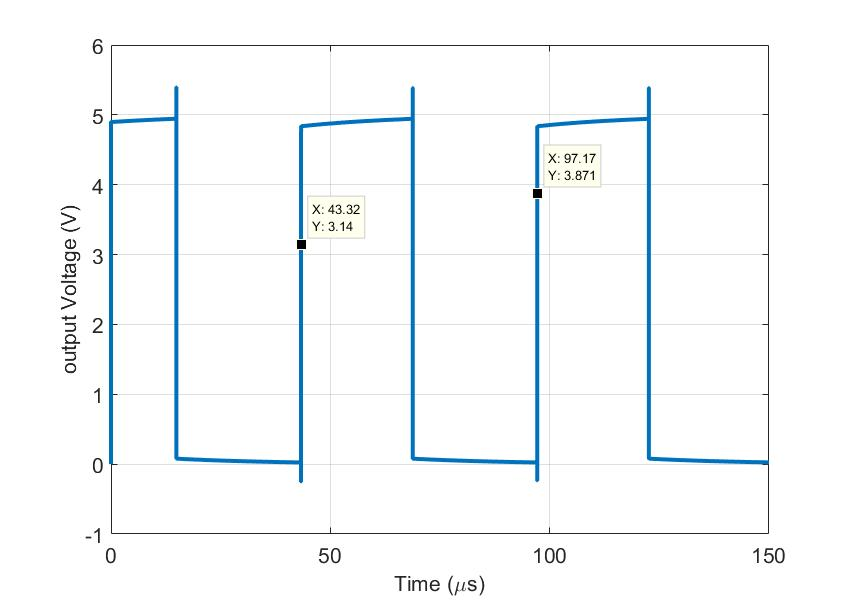
\includegraphics[scale = .35]{CircuitDevelopment/cd4007SIM/astable_DC.jpg}
        \caption{CMOS astable multivibrator output }
        \label{fig:astablesingle}
\end{figure}
Subsequently, sensitivity testing was performed on the astable multivibrator using NGSpice. First, 5\% tolerance for capacitor values was simulated, and can be seen in Figure \ref{fig:astable5percent}.

\begin{figure}[H]
    \centering
        \centering
        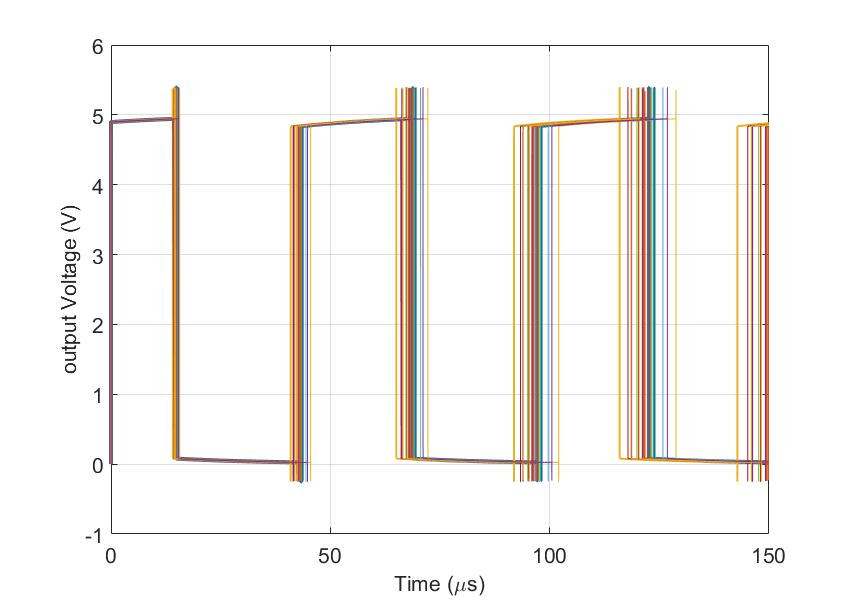
\includegraphics[scale = .35]{CircuitDevelopment/cd4007SIM/astable_5_tolerance.jpg}
        \caption{CMOS astable multivibrator - 5\% tolerance simulated}
        \label{fig:astable5percent}
\end{figure} 
This test was performed with 25 iterations, and the effect 5\% tolerance had was significant. The effect, however, is even more dramatic when 10\% tolerances are used. This can be seen in Figure \ref{fig:astable10percent}.

\begin{figure}[H]
    \centering
        \centering
        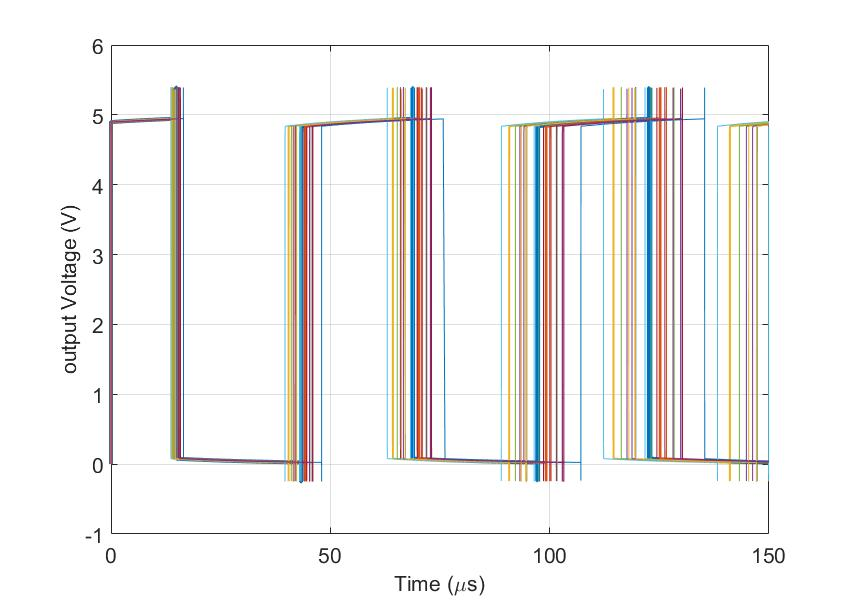
\includegraphics[scale = .35]{CircuitDevelopment/cd4007SIM/astable_10_tolerance.jpg}
        \caption{CMOS astable multivibrator  - 10 \% tolerance simulated}
        \label{fig:astable10percent}
\end{figure} 
This test was performed with 25 iterations, and tolerances can play a key role in the operating frequency.



\subsubsection{CMOS ring oscillator}

\noindent The design of the CMOS ring oscillator will consist of three CMOS inverters connected in series with the output of the last inverter connected to the input of the first inverter. The ring oscillator will also have a capacitor at each output connected to ground. The schematic for the CMOS ring oscillator can be seen in Figure \ref{fig:oscillator}.

\begin{figure}[H]
    \centering
        \centering
        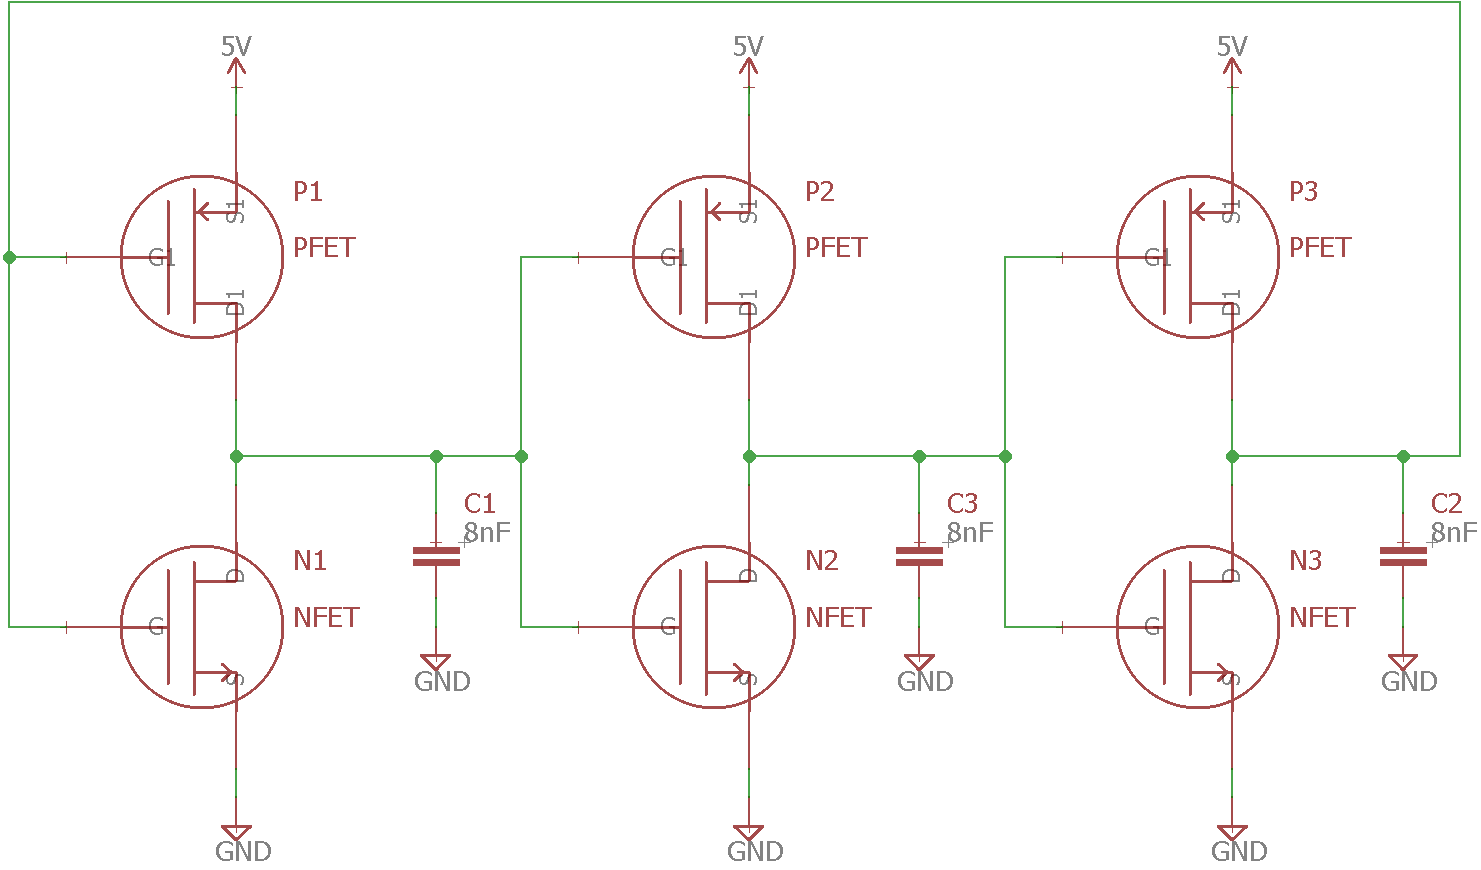
\includegraphics[scale = .3]{CircuitDevelopment/cd4007SIM/RingOscillatorCMOS.png}
        \caption{CD4007UBE ring oscillator}
        \label{fig:oscillator}
\end{figure} 

The operation of the ring oscillator uses a series of inverters. The output of one inverter inverts the input signal. Therefore, if there are a series of inverters, then each odd inverter will have the same inverted output as the first. In this instance, there are three stages of inverters used, with the output of the third inverter being fed back into the input of the first inverter. This feedback from the output to the input causes an oscillation. Based on this, it would be impossible to provide an oscillation using an even number of inverters connected in series.\newline

The ring oscillator circuit requires only a DC power source with a threshold voltage above what is required of the MOSFETS, and the oscillations will occur. To increase the frequency, the DC supply can be increase, causing an increase in current as well as frequency. \newline

The inverse of the oscillation frequency, the oscillation period, is based on the delay in each stage of the ring oscillator. The period is equivalent to double the sum of all propagation delays. These delays are caused by gates being unable to switch instantly in the real world. In this case, the gate capacitance must be charged before a connection is made between the source and the drain. Otherwise, current will be unable to flow between the source and the drain. The time it takes for the gate capacitance to reach the necessary charge adds a delay to the oscillator. Increasing the number of stages increases the delay time and reduces the frequency. The output waveform is shown in Figure \ref{fig:ringnotol}.

\begin{figure}[H]
    \centering
        \centering
        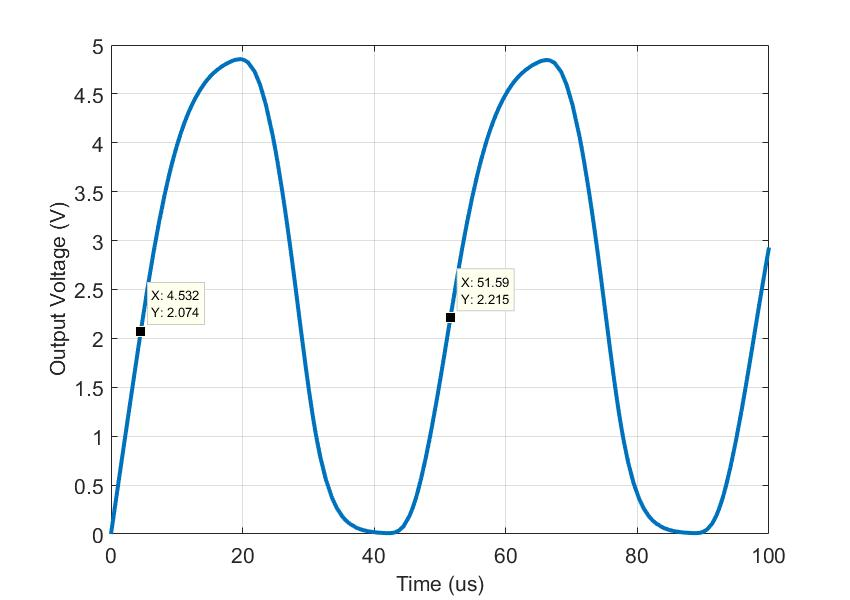
\includegraphics[scale = .35]{CircuitDevelopment/cd4007SIM/ring_output_notol.jpg}
        \caption{CD4007 ring oscillator output}
        \label{fig:ringnotol}
\end{figure}
The operating frequency was found to be approximately 20kHz. Sensitivity testing was performed on the circuit, as seen in Figure \ref{fig:ringtol5}. The simulated output based on a tolerance of $\pm$ 5\% in each of the capacitor values is shown.  \newline

\begin{figure}[H]
    \centering
        \centering
        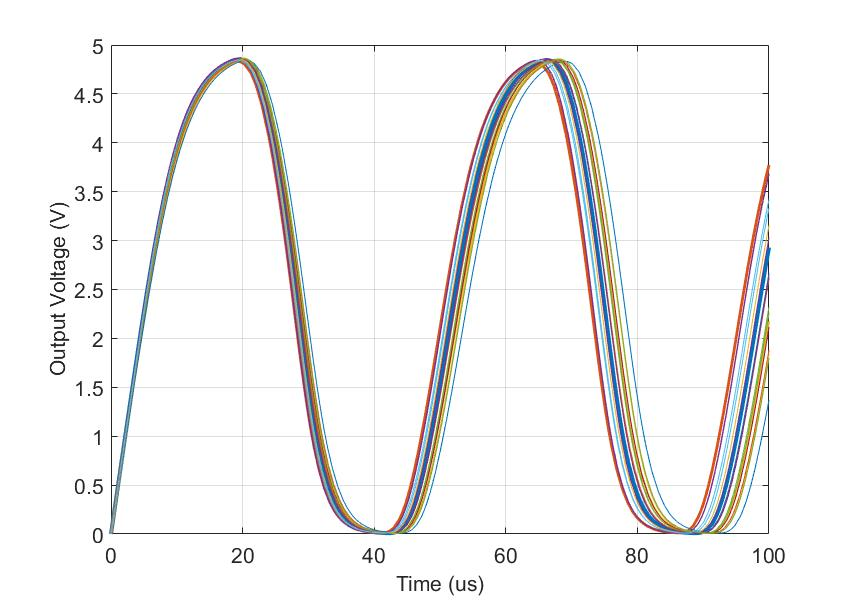
\includegraphics[scale = .35]{CircuitDevelopment/cd4007SIM/ring_5_tolerance_20it.jpg}
        \caption{CD4007 ring oscillator - 5\% tolerance simulation}
        \label{fig:ringtol5}
\end{figure}

As the simulation shows, this slight change in values has an undesired affect on the outputs. Despite only a small percentage change in capacitor values, the output of at 5\% does not stray too far from the expected output at ideal values. The simulated output in Figure \ref{fig:ringtol10}.

\begin{figure}[H]
    \centering
        \centering
        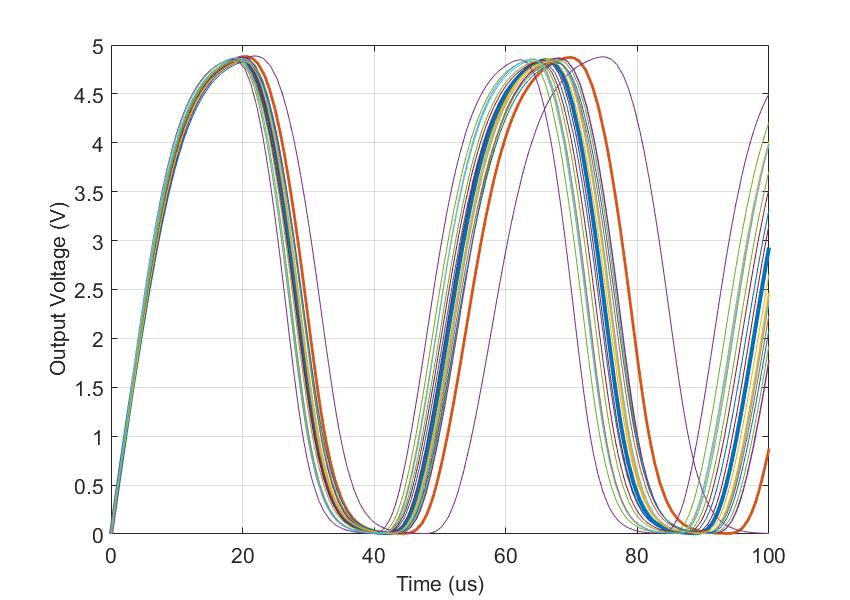
\includegraphics[scale = .35]{CircuitDevelopment/cd4007SIM/ring_10_tolerance_20it.jpg}
        \caption{CD4007 ring oscillator - 10\% tolerance}
        \label{fig:ringtol10}
\end{figure} 

As the tolerance of the capacitors in the ring oscillator increase, it causes a larger discrepancy in the values. As time goes on there are variances of almost 10$\mu s$ between simulated outputs. Based on these simulations the propagation delay caused by the gates is $\tau _P = 110ns$. The capacitor values were not calculated. Instead, the initial value of 1nF was chosen, then increased until a suitable output was found.




\end{document}